\documentclass{thesis}
\usepackage[T2A]{fontenc}
\usepackage[utf8]{inputenc}
\usepackage[english,russian]{babel}

\usepackage{fullpage}
\usepackage{lastpage}
\usepackage{enumerate}

\usepackage[all]{xy}
\usepackage{hyperref}
\usepackage[usenames,dvipsnames,svgnames,table,rgb]{xcolor}
\hypersetup{
	unicode=true,            % русские буквы в раздела PDF
	colorlinks=true,       	 % Цветные ссылки вместо ссылок в рамках
	linkcolor=black!15!blue, % Внутренние ссылки
	citecolor=blue,         % Ссылки на библиографию
	filecolor=magenta,       % Ссылки на файлы
	urlcolor=green,       % Ссылки на URL
}

\usepackage{geometry}
\geometry{left=2.5cm}
\geometry{right=1.0cm}
\geometry{top=2.0cm}
\geometry{bottom=2.0cm}
\setlength\parindent{5ex}    % Устанавливает длину красной строки 15pt
\linespread{1.3}             % Коэффициент межстрочного интервала

\newcommand{\paragraph}[1]{\noindent\textbf{#1}\quad}


%https://tex.stackexchange.com/questions/163451/total-number-of-citations
\usepackage{totcount}
\newtotcounter{citnum} %From the package documentation
\def\oldbibitem{} \let\oldbibitem=\bibitem
\def\bibitem{\stepcounter{citnum}\oldbibitem}

\makeatletter
\long\def\@makecaption#1#2{%
  \vskip\abovecaptionskip
  \sbox\@tempboxa{#1.~#2}%
  \ifdim \wd\@tempboxa >\hsize
    #1.~#2\par
  \else
    \global \@minipagefalse
    \hb@xt@\hsize{\hfil\box\@tempboxa\hfil}%
  \fi
  \vskip\belowcaptionskip}
\makeatother

\reversemarginpar

\renewcommand{\contentsname}{Содержание}
\renewcommand{\contentsdesc}{Стр.}
\renewcommand{\chaptername}{Глава}

%%% Библиография
\makeatletter
\bibstyle{utf8gost71u.bst}     % Оформляем библиографию по ГОСТ 7.1 (ГОСТ Р 7.0.11-2011, 5.6.7)
\makeatother


% Нужные мне пакеты
\usepackage{icomma}
\usepackage{amsthm}
\usepackage{graphicx}
\usepackage{amssymb}
\usepackage{amsmath}
\usepackage{graphicx}
\usepackage{color}
\usepackage{bm}
\usepackage{tabularx}
\usepackage{url}
\usepackage{multirow}
\usepackage{wrapfig}
\usepackage{caption}
\usepackage{subcaption}

% Теоремы
\newtheorem{theorem}{Теорема}
\newtheorem{lemma}{Лемма}
\newtheorem{proposition}{Утверждение}
\newtheorem*{exercise}{Упражнение}
\newtheorem*{problem}{Задача}

\newtheorem{definition}{Определение}
\newtheorem*{corollary}{Следствие}
\newtheorem*{note}{Замечание}
\newtheorem*{reminder}{Напоминание}
\newtheorem*{example}{Пример}
\newtheorem*{cexample}{Контрпример}

\newtheorem*{solution}{Решение}

\usepackage{comment}
\usepackage{rotating}

\usepackage{autonum}

\graphicspath{{./figures/}}

\begin{document}

%%% Титульный лист
\thispagestyle{empty}


\begin{titlepage}
\begin{center}
\textsc{Московский физико-технический институт}\\
(национальный исследовательский университет)\\
\textsc{Физтех-школа прикладной математики и информатики}\\
\textsc{Кафедра интеллектуальных систем}
\end{center}
\vspace{4cm}
\begin{center}
{Киселев Никита Сергеевич}
\par
\vspace{2cm}
{\Large \textsc{\textbf{Байесовский подход к выбору\\ достаточного размера выборки}}}
\par
\vspace{2cm}
{03.03.01~--- Прикладные математика и физика}
\par
\vspace{2cm}
\textsc{Выпускная квалификационная работа бакалавра}
\end{center}
\vspace{2cm}
\hfill\parbox{8,4cm}{\textbf{Научный руководитель:}
\\к.ф.-м.н. А.\,В.\,Грабовой}
\par
\vspace{3.5cm}
\begin{center}
{Москва~--- 2023}
\end{center}
\end{titlepage}
% Нумерация должна начинаться со второй страницы
\setcounter{page}{2}

%%% Аннотация
\newpage
\chapter*{Аннотация}
\begin{abstract}
	Исследуется задача выбора достаточного размера выборки. Рассматривается проблема определения достаточного размера выборки без учета природы параметров используемой модели. Предлагается использовать функцию правдоподобия выборки. Используются подходы на основе эвристик о поведении функции правдоподобия при достаточном количестве объектов в выборке. Проводится вычислительный эксперимент для анализа свойств предложенных методов.
\end{abstract}

\keywords{определение размера выборки \and байесовский подход}

%%% Оглавление
\newpage
\tableofcontents

%%% Введение
\newpage
\addcontentsline{toc}{section}{Введение}
\chapter*{Введение}
\section{Введение}

Задача машинного обучения с учителем предполагает выбор предсказательной модели из некоторого параметрического семейства. Обычно такой выбор связан с некоторыми статистическими гипотезами, например, максимизацией некоторого функционала качества. 
\begin{definition}
    Модель прогнозирования, которая соответствует этим статистическим гипотезам, называется \textbf{адекватной} моделью.
\end{definition}

При проведении эксперимента зачастую дана конечная обучающая выборка.

\begin{definition}
    Размер выборки, необходимый для построения адекватной модели прогнозирования, называется \textbf{достаточным}.
\end{definition}

В работе \cite{Grabovoy2022} представлены десять методов для оценки достаточного размера выборки. Среди них есть как статистические, так и байесовские подходы. 

%%% Основная часть
\clearpage
\chapter{Постановка задачи}\label{chap1}

Задана выборка размера $m$:
\[ \mathfrak{D}_m = \left\{ \mathbf{x}_i, y_i \right\}_{i = 1}^{m}, \]
где $\mathbf{x}_i \in \mathbb{X}, y_i \in \mathbb{Y}$.
%В случае обобщенной линейной модели $\mathbb{X} = \mathbb{R}^n$. Множество $\mathbb{Y} = \mathbb{R}$ в задаче регрессии и $\mathbb{Y} = \left\{ 1, \ldots, K \right\}$ в задаче $K$-классовой классификации.

Введем параметрическое семейство $p(y | \mathbf{x}, \mathbf{w})$ для аппроксимации неизвестного апостериорного распределения $p(y | \mathbf{x})$ целевой переменной $y$ при известных признаковом описании объекта $\mathbf{x}$ и параметрах $\mathbf{w} \in \mathbb{W}$. 
%Для обобщенной линейной модели $\mathbb{W} = \mathbb{R}^n$.

Определим функцию правдоподобия и логарифмическую функцию правдоподобия выборки $\mathfrak{D}_m$:
\[ L(\mathfrak{D}_m, \mathbf{w}) = \prod_{i=1}^{m} p(y_i | \mathbf{x}_i, \mathbf{w}), \qquad l(\mathfrak{D}_m, \mathbf{w}) = \sum\limits_{i=1}^{m} \log p(y_i | \mathbf{x}_i, \mathbf{w}). \]

Оценим параметры, используя метод максимума правдоподобия:
\[ \hat{\mathbf{w}}_{m} = \arg\max_{\mathbf{w}} L(\mathfrak{D}_m, \mathbf{w}). \]

Требуется найти достаточный размер выборки $m^*$. При этом понятие достаточности может определяться различными способами. Часто оно дается в терминах функции правдоподобия и полученной из ее максимизации оценки параметров. Также стоит учесть, что возможно $m^* \leqslant m$ или $m^* > m$. Эти два случая будут отдельно рассмотрены далее.

\clearpage
\chapter{Достаточный размер выборки не превосходит доступный}\label{chap2}

В этой главе будем считать, что достоверно $m^* \leqslant m$.

Рассмотрим выборку $\mathfrak{D}_k$ размера $k \leqslant m$. Оценим на ней параметры, используя метод максимума правдоподобия:
\[ \hat{\mathbf{w}}_{k} = \arg\max_{\mathbf{w}} L(\mathfrak{D}_k, \mathbf{w}). \]

Поскольку природа $\mathbf{w}$ нам неизвестна, для определения достаточности будем использовать функцию правдоподобия.

Когда в наличии имеется достаточно объектов, вполне естественно ожидать, что от одной реализации выборки к другой полученная оценка параметров не будет сильно меняться \cite{Joseph1997, Joseph1995}. То же можно сказать и про функцию правдоподобие. Таким образом, сформулируем, какой размер выборки можно считать достаточным.

\begin{definition}
    \label{opt-variance}
    Зафиксируем некоторое положительное число $\varepsilon > 0$. Размер выборки $m^*$ называется \textbf{D-достаточным}, если для любого $k \geqslant m^*$
    $$ D(k) = \mathbb{D}_{\mathfrak{D}_k} L(\mathfrak{D}_m, \hat{\mathbf{w}}_{k}) \leqslant \varepsilon. $$
\end{definition}
\begin{note}
    В определении~\ref{opt-variance} вместо функции правдоподобия $L(\mathfrak{D}_m, \hat{\mathbf{w}}_{k})$ можно рассматривать ее логарифм $l(\mathfrak{D}_m, \hat{\mathbf{w}}_{k})$.
\end{note}

С другой стороны, когда в наличии имеется достаточно объектов, также вполне естественно, что при добавлении очередного объекта в рассмотрение полученная оценка параметров не будет сильно меняться. Сформулируем еще одно определение.

\begin{definition}
    \label{opt-difference}
    Зафиксируем некоторое положительное число $\varepsilon > 0$. Размер выборки $m^*$ называется \textbf{M-достаточным}, если для любого $k \geqslant m^*$ 
    $$ M(k) = \left| \mathbb{E}_{\mathfrak{D}_{k+1}} L(\mathfrak{D}_m, \hat{\mathbf{w}}_{k+1}) - \mathbb{E}_{\mathfrak{D}_k} L(\mathfrak{D}_m, \hat{\mathbf{w}}_{k}) \right| \leqslant \varepsilon. $$
\end{definition}
\begin{note}
    В определении~\ref{opt-difference} вместо функции правдоподобия $L(\mathfrak{D}_m, \hat{\mathbf{w}}_{k})$ можно рассматривать ее логарифм $l(\mathfrak{D}_m, \hat{\mathbf{w}}_{k})$.
\end{note}

\textcolor{red}{Как доказать корректность этих определений? А именно, почему такой размер выборки существует?}

По условию задана одна выборка. Поэтому в эксперименте нет возможности посчитать указанные в определениях математическое ожидание и дисперсию. Для их оценки воспользуемся техникой бутстрэп. А именно, сгенерируем из заданной $\mathfrak{D}_m$ некоторое число $B$ подвыборок размера $k$ с возвращением. Для каждой из них получим оценку параметров $\hat{\mathbf{w}}_{k}$ и посчитаем значение $L(\mathfrak{D}_m, \hat{\mathbf{w}}_{k})$. Для оценки будем использовать выборочное среднее и несмещенную выборочную дисперсию (по бутстрэп-выборкам). \textcolor{red}{Как доказать <<хорошие>> свойства этих оценок?}

\clearpage
\chapter{Достаточный размер выборки больше доступного}\label{chap3}

В этой главе будем считать, что достоверно $m^* > m$.

Возникает задача прогнозирования математического ожидания и функции правдоподобия при $k > m$. \textcolor{red}{Как определить характер этой зависимости?}



\clearpage
\chapter{Вычислительный эксперимент}\label{chap4}

Проводится эксперимент для анализа свойств предложенных методов оценки достаточного размера выборки. Эксперимент состоит из двух частей. В первой части рассматриваются оценки достаточного размера выборки в случае, когда достаточный размер выборки не превосходит доступный. Во второй части исследуются результаты, полученные в условиях того, что достаточный размер выборки больше доступного.

\section{Достаточный размер выборки не превосходит доступный}

Синтетические данные сгенерированы из модели линейной регрессии. Число объектов 1000, число признаков 20. Далее приведены графики логарифма функции правдоподобия выборки, а также функций $D(k)$ и $M(k)$, определенных в Главе~\ref{chap2} (здесь используется логарифм функции правдоподобия). Выполнено определение D-достаточного и M-достаточного размеров выборки. Использовалось $B=1000$ бутстрэп-выборок. Результаты представлены на Рис.~\ref{synthetic-regression-sufficient}.

\begin{figure}[h!]
    \centering
    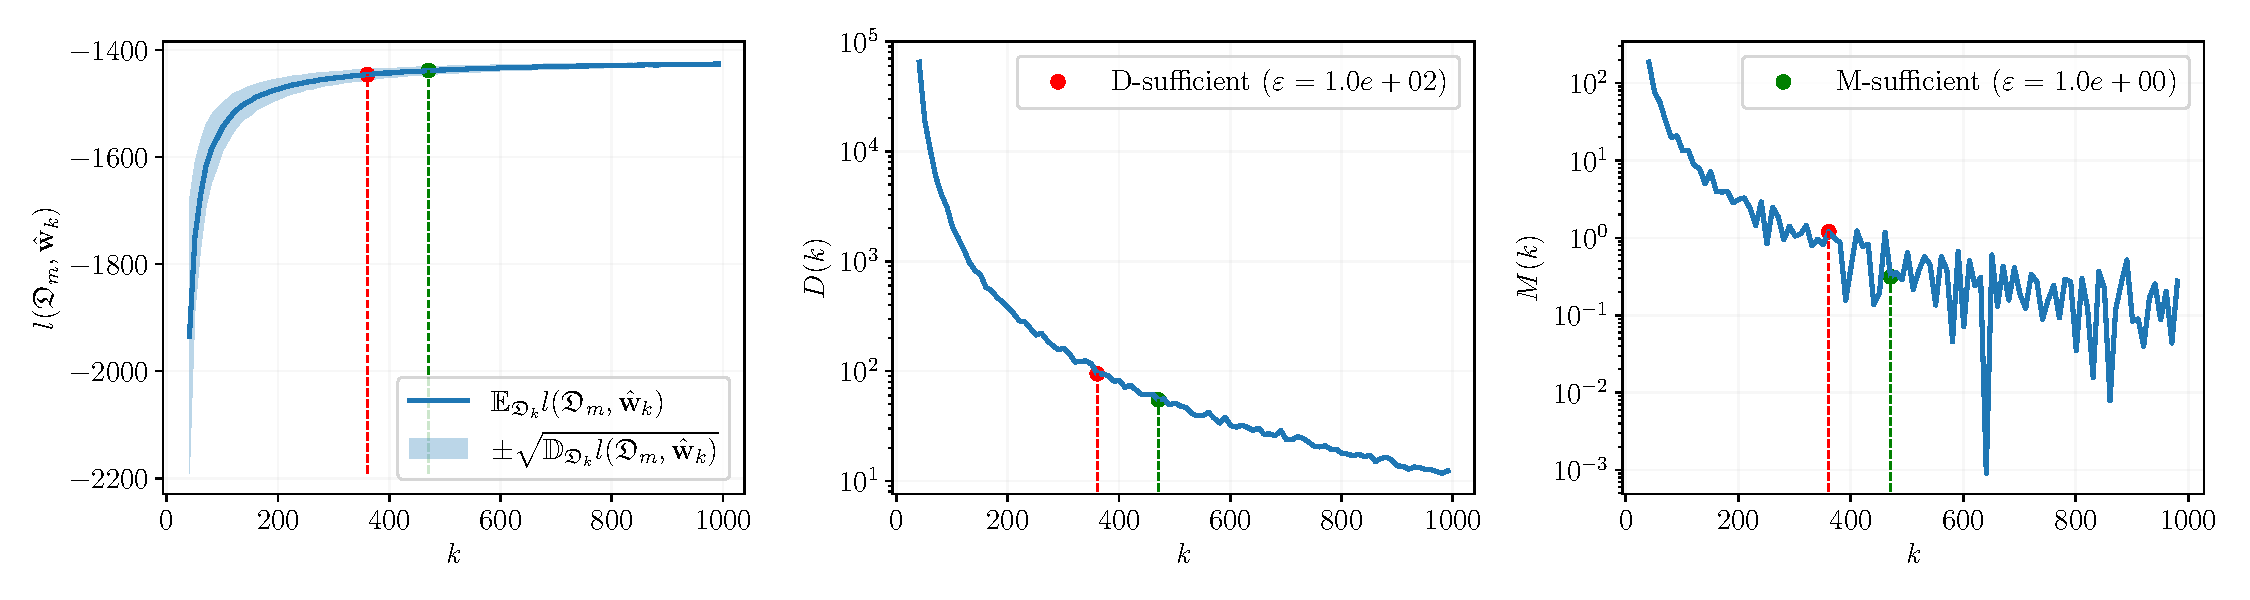
\includegraphics[width=\textwidth]{paper/figures/synthetic-regression-sufficient.pdf}
    \caption{Синтетическая выборка (линейная регрессия) при $m^* \leqslant m$}
    \label{synthetic-regression-sufficient}
\end{figure}

Вторая синтетическая выборка сгенерирована из модели логистической регрессии. Число объектов 1000, число признаков 20. Аналогичные графики приведены на Рис.~\ref{synthetic-classification-sufficient}.

\begin{figure}[h!]
    \centering
    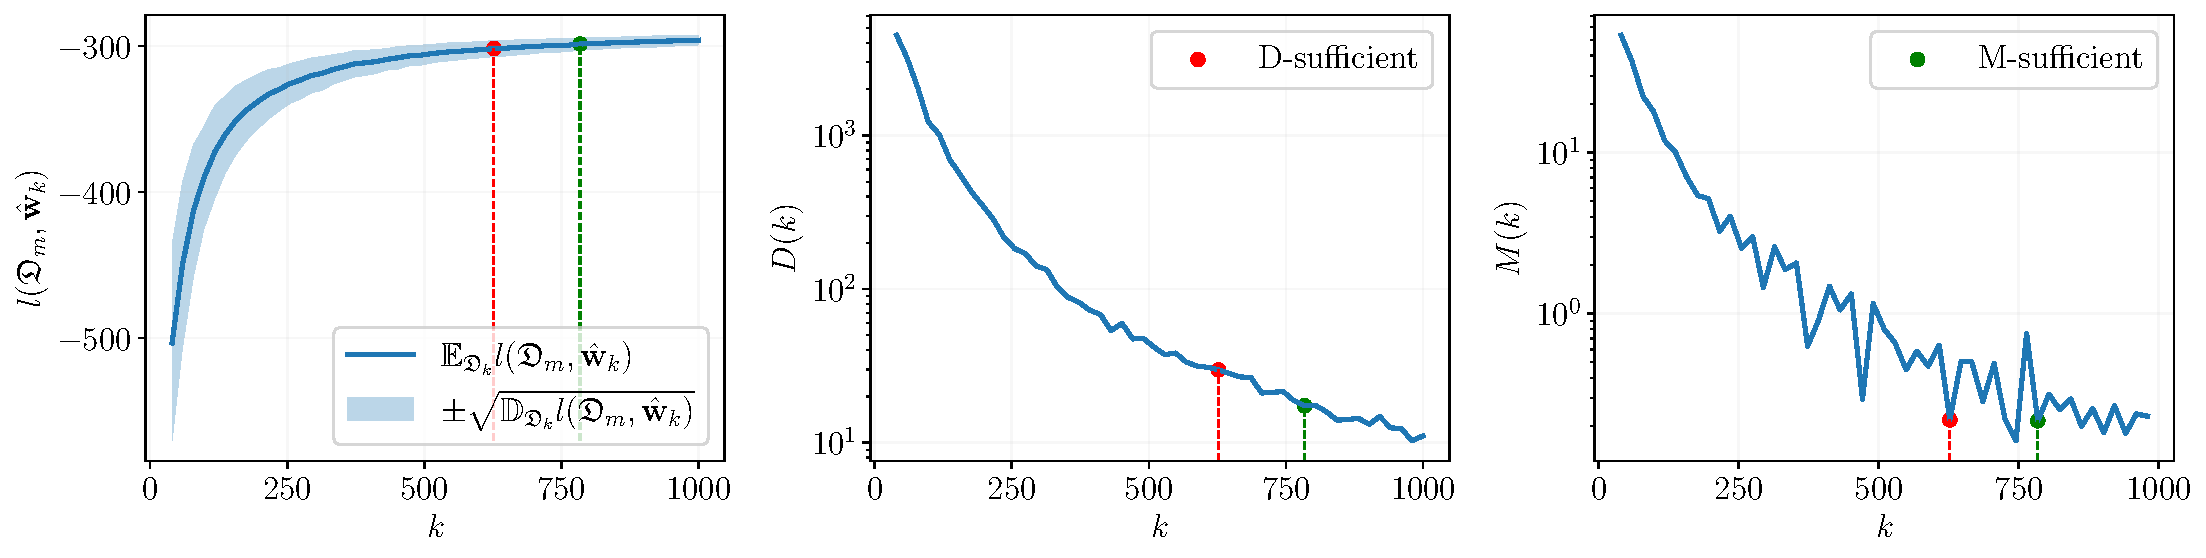
\includegraphics[width=\textwidth]{paper/figures/synthetic-classification-sufficient.pdf}
    \caption{Синтетическая выборка (логистическая регрессия) при $m^* \leqslant m$}
    \label{synthetic-classification-sufficient}
\end{figure}

\section{Достаточный размер выборки больше доступного}

Для синтетических выборок проведена аппроксимация функций правдоподобия. Среднее значение и дисперсия аппроксимированы соответственно функциями
\[ \varphi(m) = a_1 - a_2^2 \exp\left( - a_3^2 m \right) - \dfrac{a_4^2}{m^{3/2}} \]
и
\[ \psi(m) = b_1^2 \exp\left( - b_2^2 m \right) + \dfrac{b_3^2}{m^{3/2}}, \]
где $\mathbf{a}$ и $\mathbf{b}$~--- вектора параметров.

Производилось разделение на обучающую и тестовую выборки в соотношении 70:30. Аппроксимация производилась только на обучающей части. Достаточный размер выборки находился в тестовой части. На Рис.~\ref{synthetic-regression-approximation} и Рис.~\ref{synthetic-classification-approximation} представлены истинные и восстановленные зависимости. Там же указаны определенные D-достаточный и M-достаточный размеры выборки.

\begin{figure}[h!]
    \centering
    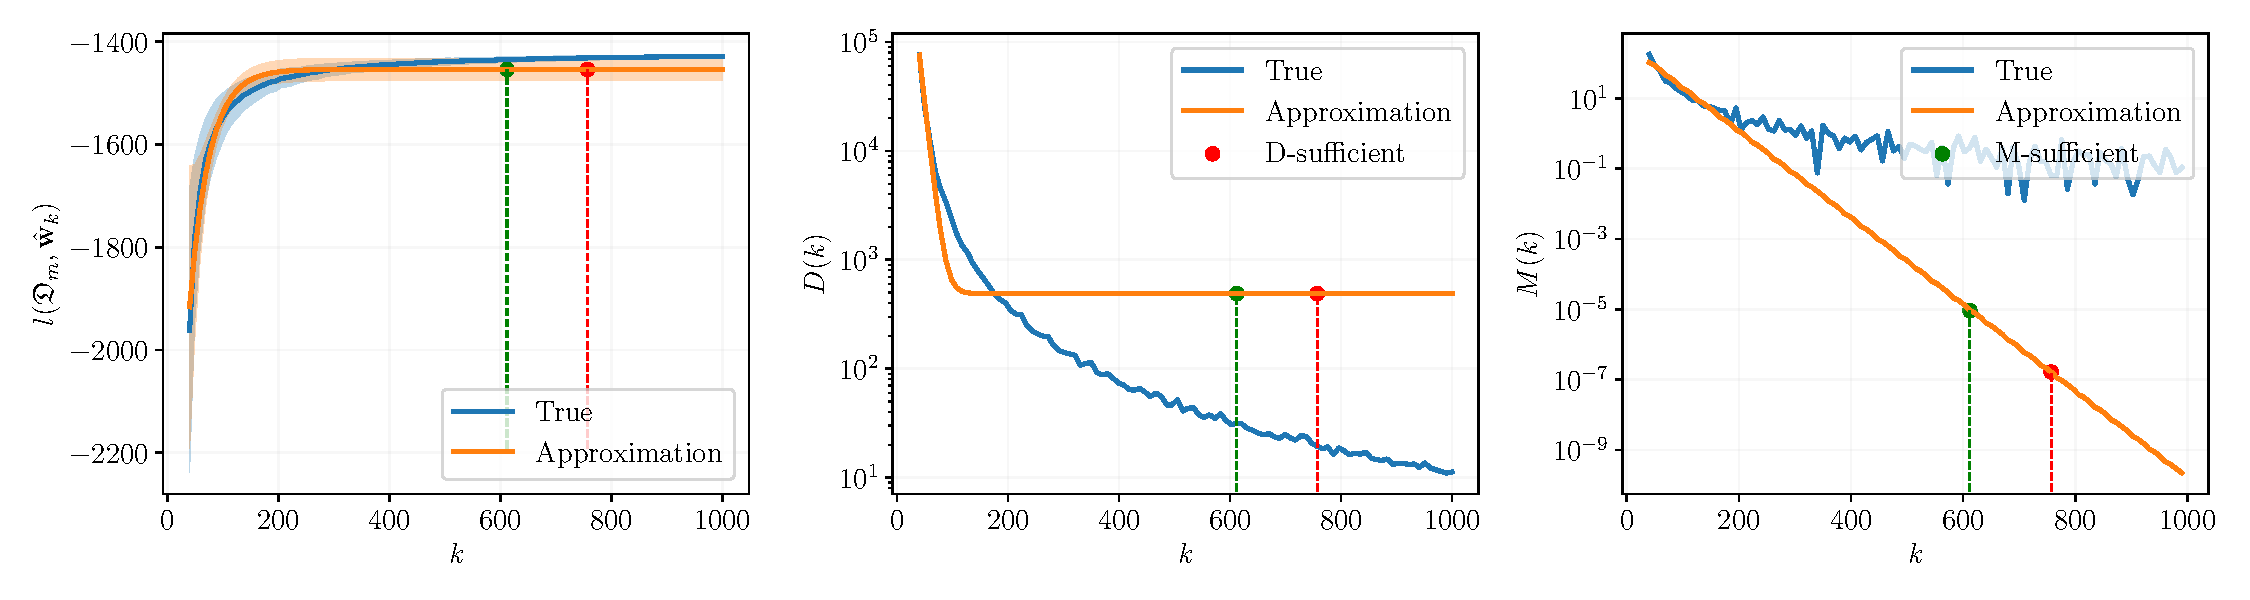
\includegraphics[width=\textwidth]{paper/figures/synthetic-regression-approximation.pdf}
    \caption{Синтетическая выборка (линейная регрессия) при $m^* > m$}
    \label{synthetic-regression-approximation}
\end{figure}

\begin{figure}[h!]
    \centering
    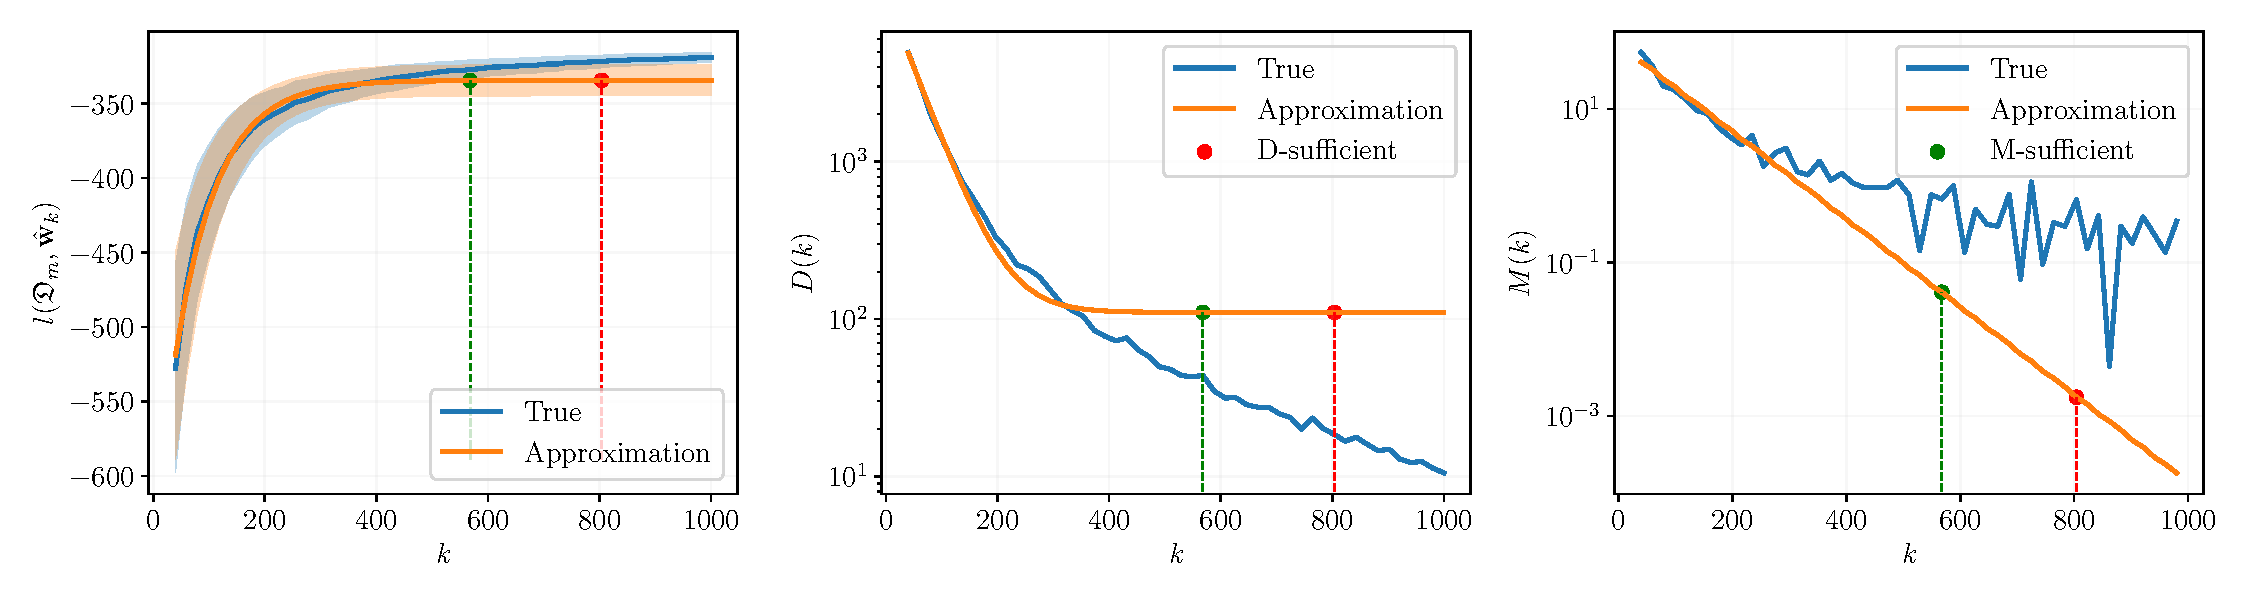
\includegraphics[width=\textwidth]{paper/figures/synthetic-classification-approximation.pdf}
    \caption{Синтетическая выборка (логистическая регрессия) при $m^* > m$}
    \label{synthetic-classification-approximation}
\end{figure}

%%% Заключение
\clearpage
\addcontentsline{toc}{section}{Заключение}
\chapter*{Заключение}
\section{Заключение}

Основные результаты данной работы заключаются в следующем. Предложены способы определения достаточного размера выборки, не использующие распределение параметров модели. Это позволяет применять их для любой модели прогнозирования, будь то линейная регрессия или нейронная сеть. В частном случае доказана корректность такого определения. Проведены вычислительные эксперименты, подтверждающие теоретические выкладки и демонстрирующие работу метода.

%%% Список основных обозначений
%\clearpage
%\addcontentsline{toc}{section}{Список оcновных обозначений}
%\chapter*{Список оcновных обозначений}
%\input{notations.tex}

%%% Список иллюстраций
\clearpage 
\addcontentsline{toc}{section}{Список иллюстраций}
\listoffigures

%%% Список таблиц
%\clearpage
%\addcontentsline{toc}{section}{Список таблиц}
%\listoftables

%%% Список литературы
\clearpage
\addcontentsline{toc}{section}{Список литературы}
\renewcommand{\bibname}{Список литературы}
\nocite{*}
%\bibliography{references.bib}
\bibliographystyle{abbrv}
\bibliography{references.bib}


%%% Приложения
%\input{appendices.tex}

\end{document}